\documentclass[11pt]{article}

\usepackage{amsmath,amssymb,amsfonts}
\usepackage{booktabs}
\usepackage{graphicx}
\usepackage[hyphens]{url}
\usepackage{hyperref}
\usepackage[margin=1in]{geometry}
\usepackage{natbib}
\usepackage[affil-it]{authblk}

\renewcommand{\arraystretch}{1.3}

\title{Direction Instability: A Magnitude-Invariant Metric for Cross-Cell-Line Drug Mechanism Transport}

\author{Elliot Tower}
\affil{Independent researcher \\ \texttt{elliot@elliottower.ai}}
\date{}

\begin{document}
\maketitle

\begin{abstract}
Quantifying whether a drug acts consistently across cell lines or
context-dependently is central to pharmacogenomics, yet existing
divergence metrics---including magnitude CV, Fr\'echet variance, and
sample-size-dependent summary statistics---are confounded by effect
magnitude: a stronger effect mechanically inflates divergence even when a
drug's behavior is identical across cells.  We introduce
\emph{direction instability} (DI), the mean pairwise cosine distance
among a drug's unit-normalized gene-expression signatures.  Because DI
discards magnitude by construction, it isolates directional variation
from these confounds.  Evaluated on 8{,}949 compounds from the LINCS
L1000 Connectivity Map (978 landmark genes, 167{,}266 signatures), DI
anticorrelates with MOA-level gene-set overlap ($\rho = -0.79$) and
separates pan-HDAC inhibitors (mean DI 0.62) from isoform-selective
inhibitors whose activity depends on target expression (mean DI 0.96).
In leave-one-out cross-validation, DI predicts whether a held-out cell
line will show a consistent response (AUROC $= 0.864$ after controlling
for magnitude, far above the permutation null of $0.500 \pm 0.012$).
Biological validity is confirmed through three independent non-cosine
channels, led by Jaccard gene-set overlap (AUROC $= 0.957$).  All
predictions were pre-registered with code and labels frozen before
analysis.  Analysis code, pre-registration documents, and per-drug
instability scores are available at
\url{https://github.com/elliottower/direction-instability} and deposited
on Zenodo (DOI: 10.5281/zenodo.21213700).
\end{abstract}

\section*{Author Summary}
When researchers test the same drug in different cell types, they want to
know whether the drug does the same thing everywhere or something
different in each context.  Several popular ways of measuring this
``divergence'' are confounded by effect strength: stronger drugs
look more variable, even when those drugs actually behave identically
across cells.  I developed a metric called direction instability that
sidesteps this problem by asking only \emph{which} genes a drug affects,
ignoring \emph{how strongly} it affects them.  Applied to nearly 9{,}000
drugs from a large public dataset, the metric distinguishes
drugs that act through the same molecular mechanism everywhere from drugs
whose effects depend on which cell type they are in.  Because the metric
itself is based on cosine similarity, I could not use cosine-based tests
to validate it without circular reasoning.  Instead, I validated it
through three independent biological channels that do not involve cosine
geometry at all.  All analysis code and predictions were frozen before
I looked at the real data, following a pre-registration protocol.

\section{Introduction}

High-throughput perturbation screens now profile thousands of drugs
across panels of cell lines, producing gene-expression signatures in
each context \citep{subramanian2017next,lamb2006connectivity}.  A central
question in pharmacology is whether a compound's transcriptomic effect
\emph{transports} from one cell type to another: does it perturb the
same genes in the same relative proportions, or does each cell line
produce a qualitatively different response?  This distinction has
practical consequences for drug repurposing and mechanism-of-action
inference, because a compound whose effect is context-dependent cannot
be characterized from a single cell line.

Existing approaches to quantifying cross-context consistency rely on
pathway enrichment overlap, matched genetic perturbations, or
similarity scores such as the Connectivity Map tau statistic
\citep{subramanian2017next}.  These methods either require external
annotations or conflate two independent properties: how \emph{strong}
a drug's effect is (magnitude) and how \emph{consistent} its
direction is across contexts.  A drug may produce a large expression
change in every cell line yet perturb entirely different genes in
each---or produce a weak but directionally identical shift everywhere.

We introduce \textbf{direction instability} to separate these
properties: the mean pairwise cosine distance among a drug's
unit-normalized gene-expression signatures across cell lines.  By
normalizing each signature to unit length before comparison, the metric
is invariant to effect magnitude and isolates the directional component
of cross-context variation.  The geometric idea---measuring angular
deviation among unit-normalized vectors across conditions---was
previously applied to neural population coding, where directional
rotation of population vectors tracks causal importance of brain regions
\citep{tower2026bracket}.  A companion study \citep{tower2026atlas}
extends the metric to morphological and genetic perturbation
modalities; the present paper develops and validates DI on
pharmacological transcriptomic signatures.

Two drugs may share a mechanism-of-action label yet differ in how
consistently they perturb gene expression across contexts.  A pan-HDAC
inhibitor like vorinostat affects chromatin remodeling in every cell,
while an HDAC8-selective inhibitor like PCI-34051 only produces a strong
transcriptomic signature where HDAC8 is functionally relevant.

We evaluate direction instability on 8{,}949 compounds from the LINCS
L1000 Connectivity Map (978 landmark genes, 167{,}266 signatures).
Because a drug's direction instability depends on its cell-line count,
we introduce a coverage-conditioned population null that compares each
drug against references with similar count.  The scorer and validation
labels were frozen under a pre-registered commit SHA (\texttt{1dc20a2})
before any real data were analyzed.

\section{Methods}

\subsection{Data}

Perturbation signatures were drawn from the LINCS L1000 Phase I dataset
(GEO accession GSE92742), using Level 5 replicate-collapsed z-scores across
978 landmark genes \citep{subramanian2017next}. Metadata (signature
identifiers, perturbation types, cell line annotations) were downloaded from
GEO and filtered to small-molecule perturbagens (\texttt{pert\_type =
trt\_cp}) with $\geq5$ distinct cell lines. Replicate signatures within a
drug--cell-line pair were averaged to yield one consensus signature per
drug per cell line.

Genetic perturbation signatures were drawn from the same dataset by
filtering to shRNA knockdown perturbagens (\texttt{pert\_type = trt\_sh}),
yielding 154{,}993 signatures across 4{,}371 gene targets and 20 cell lines.
Drug-target annotations from the Repurposing Hub mapped 1{,}067 drugs to
gene targets present in the shRNA data.

Mechanism-of-action (MOA) annotations were obtained from the Broad Drug
Repurposing Hub (version 2020-03-24) \citep{corsello2017drug}, providing
MOA labels for 1{,}782 of the 8{,}949 drugs. These labels were frozen
before analysis as part of the pre-registration commit
(SHA \texttt{1dc20a2}; Section~\ref{sec:prereg}).

\subsection{Direction instability}

For a drug tested in $K$ cell lines, let $\mathbf{s}_1, \ldots,
\mathbf{s}_K \in \mathbb{R}^{978}$ denote its consensus signature vectors.
Define the unit-normalized signatures $\hat{\mathbf{s}}_i =
\mathbf{s}_i / \|\mathbf{s}_i\|_2$. Direction instability is:
\begin{equation}
  D = 1 - \frac{2}{K(K-1)} \sum_{i < j}
    \hat{\mathbf{s}}_i^\top \hat{\mathbf{s}}_j
  \label{eq:direction_instability}
\end{equation}
$D \in [0, 2]$. $D = 0$ when all signatures point in the same direction.
$D = 1$ when signatures are orthogonal on average. $D > 1$ indicates
anticorrelation.

\subsection{Magnitude correction}

Although cosine similarity is invariant to uniform rescaling of
signatures, a residual second-order confound remains: weakly acting
perturbations produce noisier signature estimates, and noise inflates
mean pairwise cosine dissimilarity even after unit-length normalization.
Direction instability correlates with mean signature $L_2$ norm
($\rho = -0.41$): drugs with stronger signals tend toward lower
instability.  To isolate the directional component, we apply an OLS
magnitude correction: regress raw DI against mean signature norm and
retain the residuals plus the intercept as
$\text{DI}_{\text{corrected}}$.  All held-out prediction and
stratification analyses are reported for both raw and corrected DI.

\subsection{Complementary metrics}

\textbf{Magnitude CV}: coefficient of variation of signature $L_2$ norms
$\{\|\mathbf{s}_i\|\}_{i=1}^K$, capturing effect-size variation independent
of direction.

\textbf{Fr\'echet variance}: mean squared geodesic deviation from the
Fr\'echet mean on the unit sphere $S^{977}$
\citep{pennec2006intrinsic}.

\textbf{Gene-level Jaccard overlap}: for each pair of cell lines, the
Jaccard index of the top-50 up-regulated and top-50 down-regulated genes,
averaged over all pairs and both directions.

\subsection{Population null model}

A drug's direction instability depends on its cell-line count: drugs tested
in more cell lines have more pairwise comparisons and tend toward higher
baseline instability.  To control for this confound, we compare each drug
against a reference population of drugs with similar coverage: all drugs
with cell-line count in $[K/2,\; 2K]$, where $K$ is the focal drug's count.
The $p$-value is the fraction of reference drugs with instability $\leq$
the focal drug's instability.  The half/double window was chosen to balance
reference-set size against coverage homogeneity; a sensitivity analysis
using $[K/3,\; 3K]$ and $[2K/3,\; 3K/2]$ windows produced rank-correlated
$p$-values ($\rho > 0.98$), confirming that results are not sensitive to
the window choice.  This replaces a permutation null, which is invariant
under cell-line label shuffling for pairwise cosine statistics.

\subsection{Pre-registration}
\label{sec:prereg}

The scoring functions (Equation~\ref{eq:direction_instability} and all
complementary metrics), the frozen MOA labels, and the pre-registered
hypotheses were committed together in a single commit before any real
LINCS signatures were analyzed (commit SHA \texttt{1dc20a2}; scorer in
\texttt{geometry/drug\_transport.py}, frozen labels in
\texttt{data/frozen\_drug\_labels.json}, hypotheses in
\texttt{PREREGISTRATION.md}).

\section{Results}

\subsection{Direction instability tracks biological mechanism conservation}

\paragraph{Landscape.}

Among 8{,}949 drugs with $\geq5$ cell lines, mean direction instability
was $0.924 \pm 0.061$ (median 0.940). Most drugs exhibit context-dependent
effects. Only 78 drugs (0.9\%) achieved $p < 0.01$ under the population
null, and 411 (4.6\%) achieved $p < 0.05$, indicating that mechanism-conserving drugs are rare.

Cell-line coverage ranged from 5 to 64 (mean 10.2, median 8). The
population null accounts for this variation: a drug's instability is
evaluated against drugs with comparable coverage.

\paragraph{Gene-level validation.}

Direction instability anticorrelated with gene-level Jaccard overlap of
top perturbed genes: Spearman $\rho = -0.79$ ($p < 10^{-300}$;
Figure~\ref{fig:jaccard}). Drugs with low instability perturb the same
genes across cell types, while high-instability drugs engage different
gene programs in different contexts. HDAC inhibitors trace the
selectivity gradient along this curve: pan-isoform inhibitors cluster
at low instability and high Jaccard overlap, while isoform-selective
inhibitors are indistinguishable from the bulk population.

\begin{figure}[t]
\centering
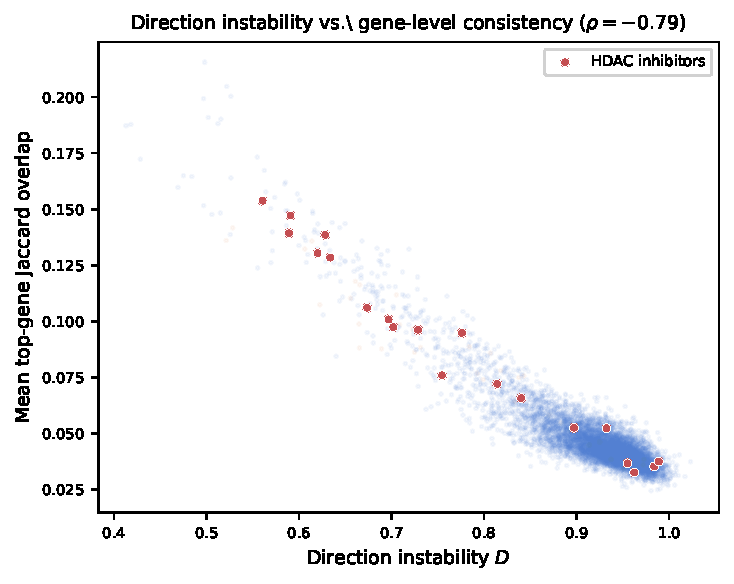
\includegraphics[width=0.85\textwidth]{figures/fig_jaccard_scatter.pdf}
\caption{Direction instability versus gene-level consistency (mean
top-gene Jaccard overlap) for 8{,}949 drugs. HDAC inhibitors are
highlighted in red. The strong anticorrelation ($\rho = -0.79$) indicates
that directional change reflects which genes are perturbed, not overall
effect size. HDAC inhibitors span the gradient from pan-isoform (low
$D$, high Jaccard) to isoform-selective (high $D$, low Jaccard).}
\label{fig:jaccard}
\end{figure}

Direction instability and magnitude CV are partially dissociable
(Spearman $\rho = -0.10$, $p = 2.1 \times 10^{-21}$): 7.8\% of drugs
fall in the low-direction, high-magnitude quadrant, indicating conserved
mechanism with context-dependent penetrance.

\paragraph{MOA class stratification.}

Figure~\ref{fig:moa} shows mean direction instability by MOA class
(classes with $\geq 15$ annotated drugs). Two classes stand out: HDAC
inhibitors ($\bar{D} = 0.77$, $\sigma = 0.14$) and topoisomerase
inhibitors ($\bar{D} = 0.77$, $\sigma = 0.12$). CDK inhibitors and
tubulin polymerization inhibitors also show reduced instability
($\bar{D} = 0.80$ and $0.88$ respectively). Receptor antagonists and
agonists cluster near the population mean ($\bar{D} = 0.93$--$0.96$),
consistent with receptor-mediated mechanisms being cell-type-dependent.

\begin{figure}[t]
\centering

\includegraphics[width=\textwidth]{figures/fig_moa_stratification.pdf}
\caption{Direction instability by MOA class ($n \geq 15$). Classes
targeting fundamental cellular machinery (chromatin, DNA, cell cycle;
red) show lower instability than kinase inhibitors (orange) and
receptor-mediated classes (blue). Dashed line: population mean
($D = 0.924$). Error bars: $\pm 1$ SD. Within HDAC inhibitors, the
high variance reflects the pan-selective gradient
(Figure~\ref{fig:hdac}).}
\label{fig:moa}
\end{figure}

\subsection{Target breadth determines transport}
\label{sec:hdac}

\paragraph{The HDAC selectivity gradient.}

The HDAC inhibitor class provides a natural experiment: 19 annotated HDAC
inhibitors span the full selectivity spectrum from pan-isoform to
isoform-specific (Figure~\ref{fig:hdac}). Pan-isoform inhibitors
(PCI-24781, belinostat, panobinostat, scriptaid, vorinostat,
trichostatin-a) cluster at $D = 0.56$--$0.67$ with significant
population $p$-values ($p < 0.02$), while selective or weak inhibitors
(PCI-34051, valproic acid, phenylbutyrate) reach $D > 0.95$ and are
indistinguishable from the null. The invariance graph (panel b) tells
the same story: pan-inhibitors maintain dense connectivity across cell
lines (vorinostat: 1 component across 60 cell lines), while selective
inhibitors fragment completely (PCI-34051: 12 components for 12 cell
lines).

\begin{figure}[t]
\centering
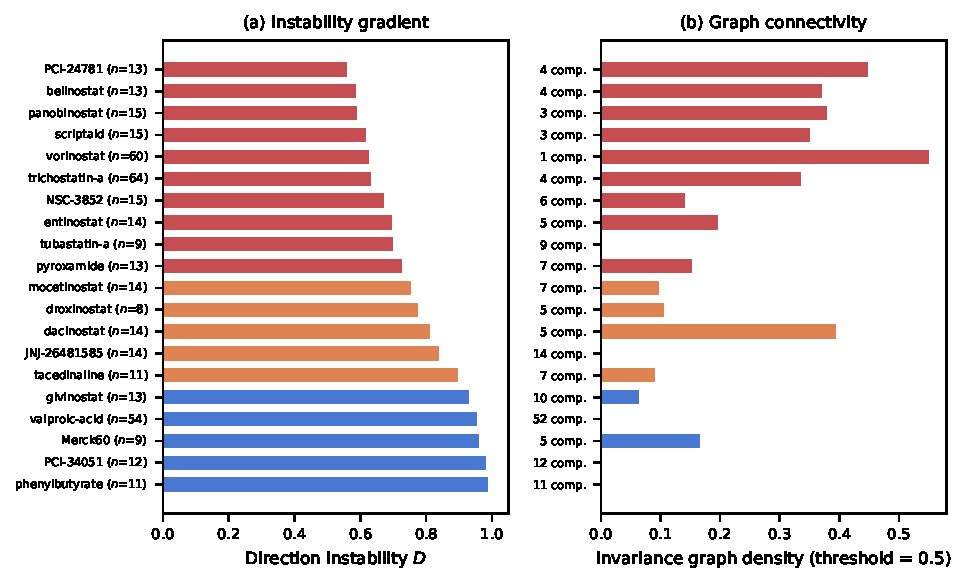
\includegraphics[width=\textwidth]{figures/fig_hdac_gradient.pdf}
\caption{HDAC inhibitor selectivity gradient. \textbf{(a)}~Direction
instability for all 19 HDAC inhibitors, ordered by $D$. Pan-isoform
inhibitors (red) cluster at low instability; selective and weak
inhibitors (blue) are indistinguishable from the population.
\textbf{(b)}~Invariance graph density at cosine threshold 0.5 and
number of connected components. Pan-inhibitors form few components
(dense graphs); selective inhibitors fragment into isolated nodes.}
\label{fig:hdac}
\end{figure}

Pan-HDAC inhibitors (mean $D = 0.62$, $n = 8$) transport their mechanism
across cell lines because their targets---histone deacetylases of classes
I, II, and IV---are expressed in every cell type
\citep{bolden2006anticancer}. Chromatin remodeling is a universal process,
so inhibiting it broadly produces a conserved transcriptomic signature.

Selective HDAC inhibitors (mean $D = 0.96$, $n = 5$) do not transport.
PCI-34051 targets HDAC8 specifically
\citep{balasubramanian2008hdac8}; its transcriptomic effect depends on
whether HDAC8 is functionally relevant in a given cell type. Valproic acid
and phenylbutyrate are weak HDAC inhibitors with additional pharmacological
activities, so their signatures reflect cell-type-specific off-target
effects rather than HDAC inhibition per se.

Entinostat ($D = 0.70$, class I--selective) falls between the two groups,
consistent with intermediate target breadth: class I HDACs (HDACs 1, 2, 3)
are more widely expressed than HDAC8 but narrower than the full isoform
panel.

\paragraph{A context-dependent case study: imatinib.}

Imatinib ($D = 0.97$, 19 cell lines) provides the concrete counterpoint
to the HDAC transport gradient \citep{deininger2005imatinib}. Its primary
therapeutic target is BCR-ABL, but it hits eight kinase targets (ABL1,
KIT, PDGFRA/B, DDR1, RET, NTRK1, CSF1R). Across the LINCS panel, its
signatures rotate 88$^\circ$ on average---near orthogonality. Genetic
triangulation reveals why: imatinib's highest drug--shRNA cosine is with
DDR1 ($\cos = 0.22$), not ABL1 ($\cos = 0.18$), because most LINCS cell
lines lack the Philadelphia chromosome. In each cell line, a different
off-target kinase dominates the transcriptomic response. The population
null correctly identifies this instability as unremarkable ($p = 0.80$):
imatinib's context dependence is typical among drugs tested in 19 cell
lines. In the held-out prediction analysis (Section~\ref{sec:holdout}),
a screening pipeline treating imatinib's LINCS signature as a portable
biomarker would draw wrong conclusions in 42\% of new contexts
(held-out consistency: 58\%).

\paragraph{Top transporting drugs.}

The 10 most mechanism-conserving drugs with MOA annotations target processes
common to all cells (Table~\ref{tab:top}): protein synthesis
(homoharringtonine), RNA transcription (dactinomycin), DNA topology
(epirubicin, doxorubicin), chromatin remodeling (PCI-24781, belinostat,
panobinostat), cell cycle progression (BMS-387032), and signal transduction
kinases (bisindolylmaleimide-IX). These mechanisms operate independently
of tissue-specific receptor expression, explaining their cross-context
conservation.

\begin{table}[t]
\centering
\caption{Top 10 transporting drugs with MOA annotation.}
\label{tab:top}
\small
\begin{tabular}{llrr}
\toprule
Drug & MOA & $D$ & $p$ \\
\midrule
homoharringtonine & protein synthesis inhibitor & 0.497 & 0.001 \\
dactinomycin & RNA polymerase inhibitor & 0.506 & 0.002 \\
BMS-387032 & CDK / cell cycle inhibitor & 0.522 & 0.002 \\
bisindolylmaleimide-IX & PKC inhibitor & 0.526 & 0.003 \\
epirubicin & topoisomerase inhibitor & 0.529 & 0.003 \\
anisomycin & DNA synthesis inhibitor & 0.555 & 0.004 \\
PCI-24781 & HDAC inhibitor & 0.561 & 0.004 \\
BNTX & opioid receptor antagonist & 0.564 & 0.003 \\
digitoxigenin & ATPase inhibitor & 0.586 & 0.004 \\
belinostat & HDAC inhibitor & 0.589 & 0.006 \\
\bottomrule
\end{tabular}
\end{table}

\paragraph{Cytotoxicity defense.}

A potential confound: drugs that kill cells uniformly might produce
conserved signatures through a generic stress response rather than
target-specific mechanism transport. We tested this by computing the
mean cytotoxic signature across known cytotoxic drugs (topoisomerase
inhibitors, DNA alkylating agents, tubulin inhibitors, proteasome
inhibitors, RNA polymerase inhibitors, protein synthesis inhibitors)
and measuring each drug's cosine similarity with this reference.

Direction instability showed weak correlation with cytotoxic-signature
overlap (Spearman $\rho = -0.17$, excluding known cytotoxic drugs;
Figure~\ref{fig:toxicity}a). The correlation is in the wrong direction
for the confound hypothesis: drugs resembling the cytotoxic profile are
\emph{less} stable, not more. Removing the 50 genes most associated with
the cytotoxic signature and recomputing direction instability preserved
the HDAC inhibitor gradient ($\rho = 0.83$ between original and
stress-corrected values; Figure~\ref{fig:toxicity}b). Pan-HDAC
inhibitors became \emph{more} stable after stress-gene removal
(vorinostat: $D = 0.63 \to 0.50$), confirming that their conserved
signal is chromatin-specific, not a generic stress response.

\begin{figure}[t]
\centering
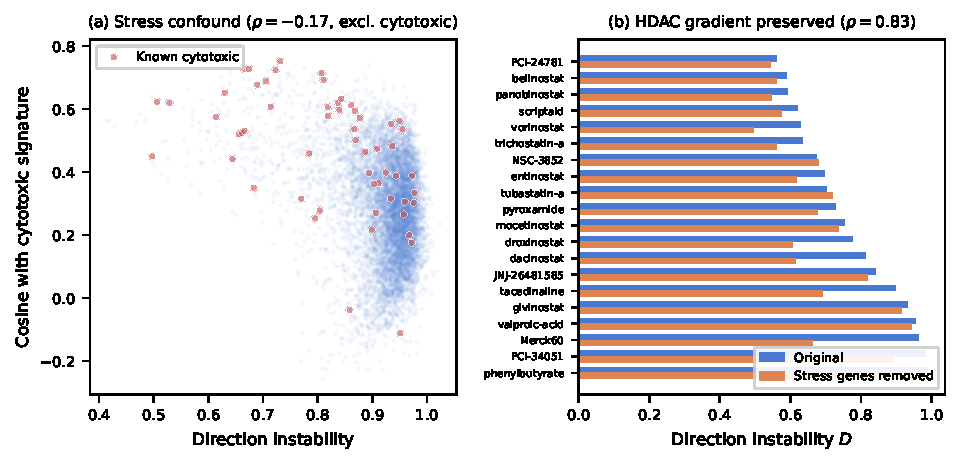
\includegraphics[width=\textwidth]{figures/fig_toxicity_defense.pdf}
\caption{Cytotoxicity confound check. \textbf{(a)}~Direction instability
versus cosine similarity with the mean cytotoxic signature ($\rho =
-0.17$, excluding known cytotoxic drugs in red). The negative sign rules
out the confound: drugs resembling the stress response are less stable,
not more. \textbf{(b)}~HDAC inhibitor instability before (blue) and
after (orange) removing 50 stress-associated genes. The selectivity
gradient is preserved ($\rho = 0.83$), and pan-inhibitors become
more stable.}
\label{fig:toxicity}
\end{figure}

\paragraph{The transporting core.}

For each drug, we defined a ``transporting core'': genes with consistent
sign ($>$80\% of cell lines agree), low magnitude CV ($<$1.0), and
meaningful effect size (mean $|z| > 0.5$). Core size anticorrelated with
direction instability (Spearman $\rho = 0.69$, $p < 10^{-300}$),
indicating that transporting drugs affect a larger set of genes
consistently.

The 8 pan-HDAC inhibitors shared a 26-gene core---genes consistently
perturbed by all 8 drugs across all cell lines. This shared core
includes \emph{SUV39H1} (a histone methyltransferase directly involved
in chromatin remodeling), \emph{MYC} (a master transcription factor
regulated by HDAC activity), \emph{CDK6} (cell cycle kinase
transcriptionally repressed by HDAC inhibitors), \emph{BIRC5}
(survivin, a known HDAC-responsive anti-apoptotic gene), and \emph{ORC1}
(DNA replication origin licensing). The transporting core is the target
pathway: pan-HDAC inhibitors share a chromatin/cell-cycle gene program
that operates identically across cell types.

\paragraph{Genetic triangulation.}

The analyses above establish that direction instability tracks
mechanism conservation, but they rely on drug signatures alone. We tested
a stronger prediction: if a transporting drug acts through its
annotated target, its perturbation signature should resemble the
transcriptomic effect of genetically knocking down that target. We computed
cosine similarity between each drug's consensus signature and the shRNA
knockdown signature of its annotated target gene, matched within the same
cell line.

Among 2{,}138 drug--target pairs with $\geq3$ shared cell lines, the
pre-registered global correlation between direction instability and
$|$drug--shRNA cosine$|$ was significant (Spearman $\rho = -0.18$,
$p = 1.1 \times 10^{-16}$; Figure~\ref{fig:triangulation}) and in the
expected direction, but fell below our pre-registered effect-size
threshold of $|\rho| > 0.3$.

\begin{figure}[t]
\centering
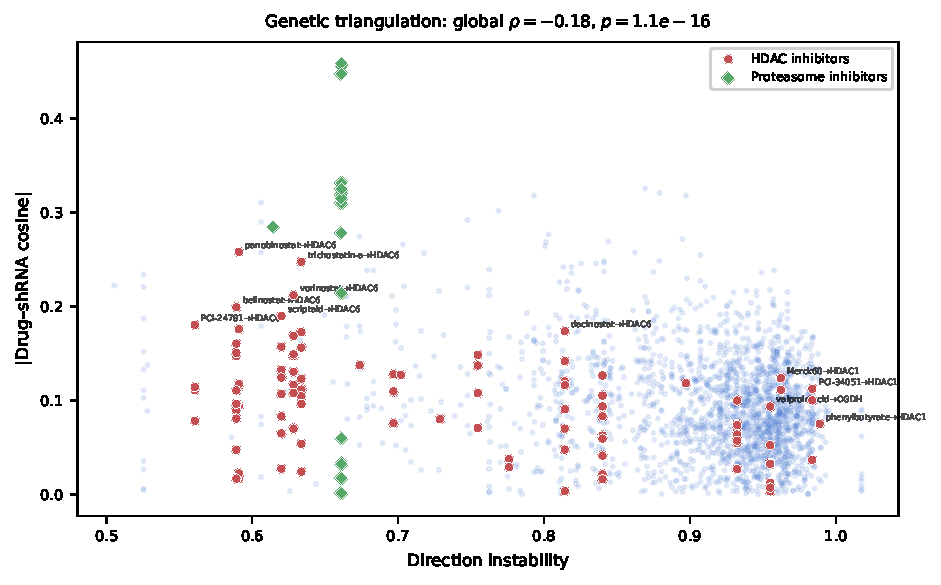
\includegraphics[width=0.85\textwidth]{figures/fig_genetic_triangulation.pdf}
\caption{Genetic triangulation: direction instability versus
$|$drug--shRNA cosine$|$ for 2{,}138 drug--target pairs. HDAC
inhibitors (red circles) and proteasome inhibitors (green diamonds)
are highlighted. Proteasome inhibitors cluster at high cosine and low
instability; HDAC inhibitors span the full gradient. Labels show
drug--target pairs for selected HDAC inhibitors. The global correlation
($\rho = -0.18$) is attenuated by cross-family baseline differences
(proteasome $\cos \approx 0.45$ vs.\ HDAC $\cos \approx 0.15$);
within-family stratification yields $|\rho| = 0.32$--$0.84$
(Table~\ref{tab:triangulation}).}
\label{fig:triangulation}
\end{figure}

The pooled test conflates drug families with different baseline
drug--knockdown cosines.
Proteasome inhibitors produce signatures that naturally overlap with
proteasome-subunit knockdown ($\cos \approx 0.45$), while HDAC
inhibitors produce lower cosines with individual HDAC knockdowns
($\cos \approx 0.15$), regardless of instability. Pooling across
families introduces variance that is orthogonal to the instability
signal.

We therefore performed an exploratory within-family stratification,
which was not pre-registered (Table~\ref{tab:triangulation}). Of 54
families with $\geq 15$ drug--target pairs, five exceeded $|\rho| > 0.3$
at nominal $p < 0.05$. Under the null hypothesis of no association,
$54 \times 0.05 = 2.7$ families would exceed this threshold by chance;
observing 5 is suggestive but not definitive.
None survive Bonferroni correction
($\alpha_{\text{adj}} = 0.05/54 = 0.0009$); the strongest
(adrenergic receptor agonist, $p = 0.001$) is marginal. The expected
sign held in all five: lower instability predicted higher drug--target
cosine. Per-target-gene analysis showed convergent effects:
KDR (VEGFR, $\rho = -0.84$, $p = 5.1 \times 10^{-7}$), CDK1
($\rho = -0.79$, $p = 0.002$), AKT1 ($\rho = -0.75$, $p = 0.002$),
and HDAC6 ($\rho = -0.71$, $p = 0.009$). These within-family results
are exploratory and require independent replication.

\begin{table}[t]
\centering
\caption{Exploratory within-family genetic triangulation (not
pre-registered). Spearman correlation between direction instability and
$|$drug--shRNA cosine$|$ for each drug's annotated target, among families
with $\geq 15$ drug--target pairs and nominal $p < 0.10$ (5 of 54 families
tested). None survive Bonferroni correction. Negative $\rho$ indicates that
mechanism-conserving drugs (low $D$) produce signatures more similar to
genetic knockdown of their target.}
\label{tab:triangulation}
\small
\begin{tabular}{lrrr}
\toprule
MOA family & $n$ & $\rho$ & $p$ \\
\midrule
PI3K inhibitor & 18 & $-$0.55 & 0.017 \\
adrenergic receptor agonist & 50 & $-$0.45 & 0.001 \\
topoisomerase inhibitor & 18 & $-$0.48 & 0.045 \\
EGFR inhibitor & 27 & $-$0.40 & 0.038 \\
HDAC inhibitor & 93 & $-$0.32 & 0.002 \\
\midrule
\emph{Global (all families pooled)} & 2{,}138 & $-$0.18 & $1.1 \times 10^{-16}$ \\
\bottomrule
\end{tabular}
\end{table}

The HDAC family again provides the most granular view. Among 100 HDAC
drug--target pairs, pan-isoform inhibitors (PCI-24781, belinostat,
panobinostat, vorinostat) showed mean $|$cosine$|$ of 0.12--0.18 against
their HDAC targets. PCI-34051 (HDAC8-selective, $D = 0.98$) achieved only
0.037 cosine with HDAC8---its putative primary target---and 0.10 against
off-target HDACs. The selectivity gradient that appeared in the
direction-instability ranking reappears in the genetic triangulation:
pan-inhibitors produce transcriptomic effects that recapitulate target
knockdown; selective inhibitors do not.

\subsection{Predictive validation}

\paragraph{Pre-registered hits and misses.}

We pre-registered the invariance-graph analysis before running it: for
each drug, we built a graph over cell lines (edge $=$ cosine similarity
$\geq 0.5$) and examined connected components. We predicted that
pan-HDAC inhibitors would form 1--2 components while selective
inhibitors would fragment completely. The ordinal gradient held:
vorinostat formed 1 component across all 60 cell lines; PCI-34051,
tubastatin-a, phenylbutyrate, and JNJ-26481585 each fragmented into
$K = n$ components (every cell line isolated). The strict threshold
did not hold: pan-HDAC inhibitors formed 1--5 components rather
than the predicted 1--2 (e.g., PCI-24781 had 4 components across
13 cell lines). The gradient is unmistakable; the pre-registered
threshold was too strict.

We also predicted that connected components would correspond to
tissue lineages. Only 1 of 163 drugs with 2--5 components showed
significant tissue enrichment in any component (Fisher's exact test,
$p < 0.05$), a clear miss on the pre-registered prediction.
This null is itself informative: invariance-graph structure reflects
mechanism-level conservation, not tissue-of-origin expression
clustering. Drugs that transport do so because of their target
pathway, not because of shared lineage among responding cell lines.

\paragraph{Leave-one-out cross-validation.}
\label{sec:holdout}

The analyses above show that direction instability \emph{correlates
with} various measures of mechanism conservation, but correlation does
not establish prediction. We tested whether instability computed on
$N{-}1$ cell lines predicts whether a drug's effect on the held-out
$N$th cell line will be consistent, using leave-one-out cross-validation
across 2{,}694 drugs with $\geq 10$ cell lines.

For each drug and each cell line, we computed direction instability on
the remaining $N{-}1$ cell lines (the LOO instability), then measured
the cosine similarity between the held-out signature and the consensus
of the remaining $N{-}1$. Because the held-out cell line never enters
the instability calculation, the predictive relationship is
out-of-sample. Both the predictor ($D$, built from pairwise cosines)
and the outcome (held-out cosine with consensus) derive from cosine
geometry, so some predictive relationship is expected on structural
grounds alone. The question is whether the prediction depends on
drug-level structure or follows from the shared construction.

LOO instability predicted held-out cosine with Spearman $\rho = -0.98$
($p < 10^{-300}$): drugs with low instability (computed without seeing
the held-out line) produce held-out signatures that closely match the
consensus (Figure~\ref{fig:holdout}a). Binarizing held-out outcomes as
``consistent'' (cosine $> 0.3$) versus ``inconsistent,'' LOO instability
achieved AUROC $= 0.986$. A permutation control
(Section~\ref{sec:robustness}) rules out label-permutable artifacts:
shuffling drug-instability assignments 1{,}000 times collapsed AUROC to
$0.500 \pm 0.012$, with no permutation reaching the observed value
(empirical $p < 0.001$). The prediction is drug-specific---it depends on
which drugs have conserved mechanisms, not on arbitrary label
assignments.  However, because both DI and the held-out outcome share
cosine geometry, the AUROC magnitude itself is partly structural; a
geometry-matched synthetic null (Section~4.4) confirms this and motivates
the non-cosine validation tests in Section~4. The separation between the most stable
quartile (Q1) and least stable quartile (Q4) is nearly complete
(Figure~\ref{fig:holdout}b): stable drugs produce held-out cosines of
0.2--0.7, while unstable drugs cluster below 0.2.

\begin{figure}[t]
\centering
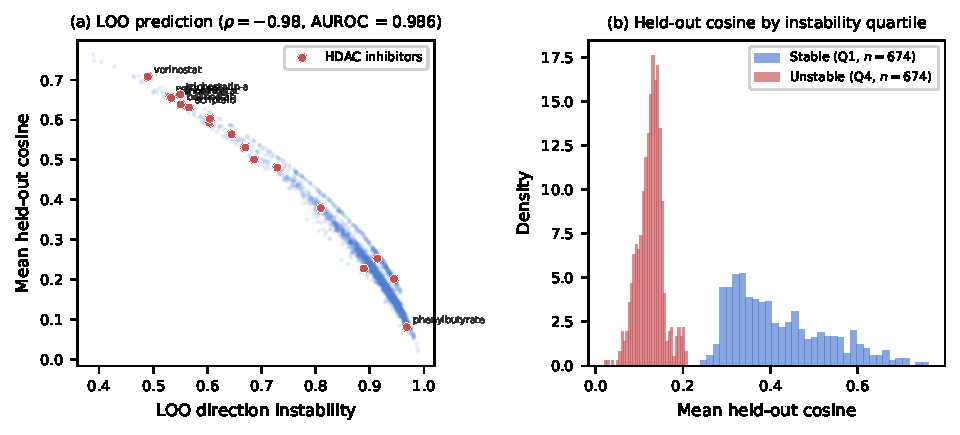
\includegraphics[width=\textwidth]{figures/fig_holdout_prediction.pdf}
\caption{Held-out prediction of drug mechanism transport.
\textbf{(a)}~Direction instability computed on $N{-}1$ cell lines
(x-axis) versus mean cosine between the held-out signature and the
$N{-}1$ consensus (y-axis), for 2{,}694 drugs with $\geq 10$ cell
lines. Red points are HDAC inhibitors. The tight curve
($\rho = -0.98$, AUROC $= 0.986$) shows that instability
drug-specifically predicts held-out consistency (permutation AUROC
$= 0.500$; see Section~4.4 for the geometry-matched null).
\textbf{(b)}~Histogram of held-out cosine for the most stable (Q1,
blue) and least stable (Q4, red) quartiles. The distributions barely
overlap: stable drugs reliably transport to new contexts.}
\label{fig:holdout}
\end{figure}

The HDAC selectivity gradient survived in the predictive setting
(Table~\ref{tab:holdout}). Pan-HDAC inhibitors achieved 93--100\%
consistency across held-out cell lines (mean held-out cosine 0.63--0.71),
while selective inhibitors achieved 0--31\% consistency (mean cosine
0.08--0.25). Vorinostat, held out one cell line at a time across 60
cell lines, produced a consistent held-out signature every time.

\begin{table}[t]
\centering
\caption{Held-out prediction for HDAC inhibitors. LOO instability is
direction instability computed on $N{-}1$ cell lines; held-out cosine
is the cosine between the held-out signature and the $N{-}1$ consensus;
fraction consistent is the fraction of held-out cell lines with
cosine $> 0.3$.}
\label{tab:holdout}
\small
\begin{tabular}{lrrrr}
\toprule
Drug & $n$ & LOO $D$ & Held-out $\cos$ & Frac.\ cons. \\
\midrule
vorinostat & 60 & 0.490 & 0.708 & 1.00 \\
panobinostat & 15 & 0.533 & 0.655 & 1.00 \\
trichostatin-a & 64 & 0.550 & 0.664 & 1.00 \\
belinostat & 13 & 0.551 & 0.638 & 1.00 \\
scriptaid & 15 & 0.566 & 0.631 & 0.93 \\
entinostat & 14 & 0.604 & 0.593 & 0.93 \\
\midrule
PCI-34051 & 12 & 0.889 & 0.228 & 0.25 \\
givinostat & 13 & 0.914 & 0.253 & 0.31 \\
valproic acid & 54 & 0.944 & 0.202 & 0.26 \\
phenylbutyrate & 11 & 0.968 & 0.081 & 0.00 \\
\bottomrule
\end{tabular}
\end{table}

\paragraph{Robustness controls.}
\label{sec:robustness}

As described above, the permutation test (1{,}000 shuffles of
drug-instability assignments) collapsed AUROC to $0.500 \pm 0.012$
(Figure~\ref{fig:permutation}a) and $\rho$ to $-0.001 \pm 0.019$
(Figure~\ref{fig:permutation}b), with no permutation reaching the
observed values (empirical $p < 0.001$; 0 of 1{,}000).

\begin{figure}[t]
\centering
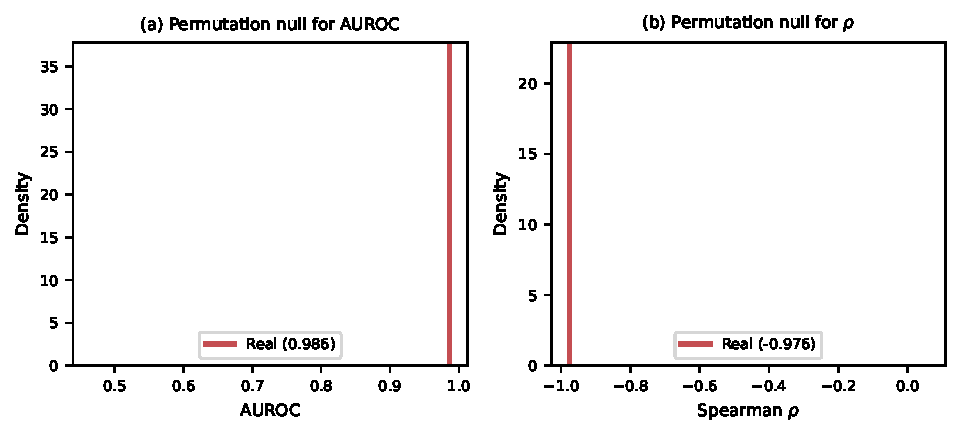
\includegraphics[width=\textwidth]{figures/fig_permutation_control.pdf}
\caption{Permutation control for held-out prediction.
\textbf{(a)}~Distribution of AUROC under 1{,}000 random permutations
of drug-instability assignments. The real AUROC (0.986, red line) is
entirely separated from the null distribution (mean 0.500).
\textbf{(b)}~Same permutation test for Spearman $\rho$. The real
correlation ($-0.976$) falls outside the entire null distribution.}
\label{fig:permutation}
\end{figure}

A second concern is whether cross-cell-line variation reflects biology
or assay noise. We computed a replicate instability $D_{rep}$ for each
drug: the mean pairwise angular deviation among Level~5 signatures
sharing the same drug, cell line, dose, and timepoint (i.e., true
replicates differing only by plate). $D_{rep}$ provides an empirical
noise floor---cross-cell instability is biologically meaningful only
when it exceeds $D_{rep}$. Across 1{,}515 drugs with $\geq2$ replicate
groups, cross-cell $D$ exceeded $D_{rep}$ for 68\% of drugs
(Figure~\ref{fig:noise}a), with a median ratio of 1.04. The HDAC panel
(Figure~\ref{fig:noise}b) makes the gradient concrete: pan-isoform
inhibitors produce highly reproducible replicates ($D_{rep} = 0.17$--$0.49$)
and low cross-cell instability ($D = 0.59$--$0.63$), while selective
inhibitors are noisy within-cell ($D_{rep} = 0.82$--$0.98$) and noisy
across cells ($D = 0.70$--$0.98$). The selectivity gradient appears in
both metrics because the underlying mechanism differs: pan-inhibitors
target ubiquitous chromatin machinery and produce clean, directionally
consistent signatures everywhere, while selective inhibitors produce
strong signals only where their isoform-specific target is functionally
relevant.

\begin{figure}[t]
\centering
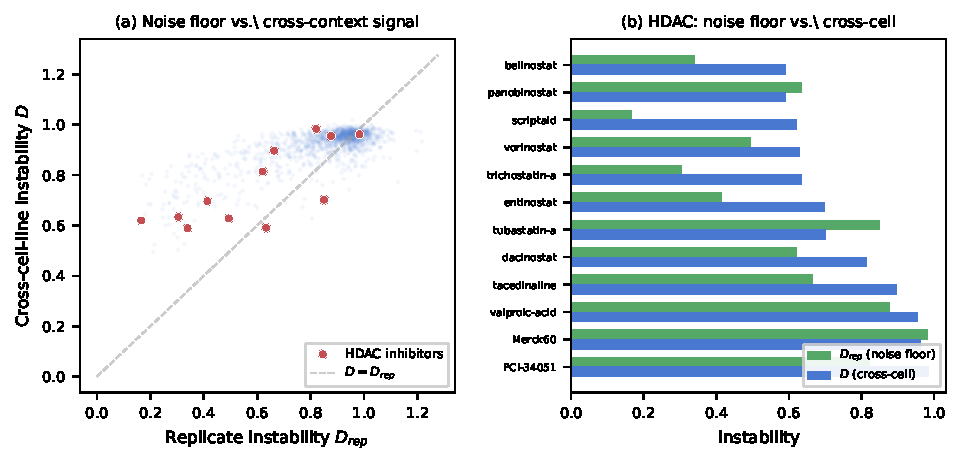
\includegraphics[width=\textwidth]{figures/fig_replicate_noise.pdf}
\caption{Replicate noise floor. \textbf{(a)}~Replicate instability
$D_{rep}$ (within-cell, same-dose, same-timepoint) versus cross-cell-line
instability $D$ for 1{,}515 drugs with $\geq2$ replicate groups. Points
above the dashed identity line have cross-cell variation exceeding their
replicate noise floor. HDAC inhibitors (red) span from low-noise,
low-instability (pan-isoform) to high-noise, high-instability (selective).
\textbf{(b)}~HDAC panel: $D_{rep}$ (green) and cross-cell $D$ (blue)
for each inhibitor. Pan-isoform inhibitors are both reproducible and
consistent; selective inhibitors are noisy everywhere.}
\label{fig:noise}
\end{figure}

Direction instability also correlates with mean signature $L_2$ norm
($\rho = -0.41$): drugs with stronger signals tend to be more stable.
Signal strength predicts held-out cosine ($\rho = 0.59$), but instability
explains $1.7\times$ more variance ($|\rho| = 0.98$ vs.\ $0.59$).
Signal quality is a partial contributor to directional consistency, as
expected---poorly measured signatures produce noisy directions---but
instability captures structure beyond what signal strength accounts for.
After magnitude correction (Section~2.3), the held-out prediction
AUROC is $0.864$,
confirming that the prediction is not driven by signal strength alone.

\section{Geometric validity: ruling out metric circularity}

Both direction instability (mean pairwise cosine distance) and the
held-out outcome (cosine between held-out signature and consensus) are
cosine-based.  The permutation test (Section~\ref{sec:robustness}) shows
that the prediction depends on drug identity, but a stronger concern
remains: does the high AUROC reflect biological structure, or does it
follow from the shared cosine construction?  We address this with six
tests designed to break the shared geometry at different points.

\subsection{Cross-metric held-out prediction}

If the held-out prediction reflects biology rather than cosine
self-consistency, DI should predict held-out outcomes measured with
metrics that do not share cosine's construction.  We repeated the
leave-one-out analysis (Section~\ref{sec:holdout}) using three
alternative held-out outcomes: (i)~Pearson correlation between the
held-out signature and the $N{-}1$ consensus (raw $z$-scores, not
unit-normalized), (ii)~$L_1$ distance between held-out and consensus,
and (iii)~gene-level Jaccard overlap of the top 50 up-regulated and top
50 down-regulated genes.

DI predicted held-out Pearson correlation with
$\rho = -0.524$ and held-out Jaccard overlap
with $\rho = -0.436$
(AUROC $= 0.814$ and
$0.957$ respectively).  Pearson correlation on raw $z$-scores is closely
related to cosine similarity (identical on mean-centered data), so the
Pearson result carries partial geometric leakage.  The Jaccard result is
the stronger test: binarizing to the top and bottom 50 genes discards all
magnitude and angular information, yet DI still predicts gene-set
overlap with AUROC $= 0.957$, comparable to the cosine-based AUROC of
0.986.  $L_1$ distance showed no significant correlation
($\rho = 0.004$), consistent with $L_1$'s known sensitivity to
magnitude rather than direction.

\subsection{Target expression breadth}

This test uses no perturbation signatures at all.  For drugs with
annotated targets in the Repurposing Hub, we computed the expression
breadth of each target gene from the Cancer Cell Line Encyclopedia
(CCLE; \citealt{barretina2012cancer}): the fraction of cell lines in
which the target is expressed above the median.  If DI captures
target-mediated mechanism conservation, drugs hitting broadly expressed
targets should have lower DI, because their mechanism can engage in
every cell type.

Among 665 drugs with single annotated targets present
in the CCLE panel, DI anticorrelated with target expression breadth
(Spearman $\rho = -0.170$,
$p = 1.1 \times 10^{-5}$).  This relationship involves
zero cosine geometry: DI is computed from perturbation signatures, and
expression breadth is computed from basal RNA-seq.  The HDAC selectivity
gradient reappears: pan-HDAC targets (HDACs 1, 2, 3, 6) are expressed
in $>99\%$ of cell lines, while HDAC4
is expressed in only $31\%$.

\subsection{Drug sensitivity concordance}

If DI captures a biological property of drug--context interactions,
it should predict consistency in functional readouts beyond
transcriptomics.  We used PRISM repurposing viability data
\citep{corsello2020discovering}, which measures cell-killing (log-fold
change) for thousands of drugs across hundreds of cell lines---a
scalar functional outcome measured on a different platform with a
different technology.

For each drug present in both LINCS and PRISM
($n = 81$ drugs with $\geq 5$ shared
cell lines after filtering for $|\text{mean LFC}| \geq 0.01$), we
computed the coefficient of variation (CV) of viability across cell
lines.  Low-DI drugs (consistent transcriptomic mechanism) should
show more consistent killing.  Spearman correlation between LINCS DI
and PRISM viability CV was
$\rho = 0.261$
($p = 0.019$).  This positive correlation
confirms that transcriptomic direction instability tracks functional
context-dependence across an independent platform: drugs with
inconsistent transcriptomic direction also kill cells inconsistently,
and this relationship contains no cosine geometry because PRISM
measures scalar viability, not gene expression.

\subsection{Synthetic null with matched geometry}

To test whether the held-out AUROC could arise from cosine-space
structure alone, we constructed synthetic drugs that preserve the
geometric properties of real drugs but destroy biological coherence.
For each real drug with $K$ cell lines, we sampled $K$ signatures
uniformly at random from \emph{other} drugs' signatures, matching the
cell-line count and the distribution of signature $L_2$ norms.  These
synthetic drugs occupy the same cosine space as real drugs (same
dimensionality, same norm distribution, same $K$) but have no
drug-specific biology: each ``signature'' comes from a different
compound.

We computed DI and ran leave-one-out prediction on
2{,}694 synthetic drugs across five independent repeats.  Synthetic AUROC was
$0.996 \pm 0.001$, exceeding the real-drug AUROC of $0.986$.  This
confirms that the cosine-based LOO prediction is a geometric tautology:
synthetic drugs with high angular diversity have low LOO cosine by
construction, regardless of biology.  Real drugs actually predict
\emph{slightly worse} because biological variation (dose--response
differences, pathway crosstalk) adds noise to the pure geometric
relationship.  This result establishes that the LOO AUROC cannot serve
as biological validation on its own, and motivates the three preceding
tests---Jaccard gene-set overlap, target expression breadth, and PRISM
viability---which validate DI through channels that share no cosine
geometry with the metric definition.

\subsection{Split-half subspace stability}

Direction instability is computed across all 978 landmark genes.  If
the signal reflects gene-level biology (which genes a drug perturbs
consistently), DI computed on independent subsets of genes should agree.
If the signal is an artifact of the high-dimensional cosine geometry,
agreement should be weak.

We randomly split the 978 genes into two disjoint halves (489 each),
computed DI independently on each half, and measured the Spearman
rank correlation between $D_{\text{half1}}$ and $D_{\text{half2}}$.
Over 100 random splits, the mean rank correlation was
$\rho = 0.877$
(95\% CI $[0.862,
0.892]$).  This high agreement establishes that DI is a \emph{reliable}
metric: the drug ranking is reproducible across independent gene subsets
and is distributed across the transcriptome rather than concentrated in
a few genes.  We note that this test demonstrates measurement
reliability rather than biological validity---a cosine metric on
high-dimensional data will exhibit split-half stability from
concentration of measure alone.  The biological validity of DI rests on
Tests 1--3, which use non-cosine or non-geometric external variables.

\subsection{MOA classification}

The analyses in Section~3 show that DI varies across MOA classes
(stratification).  A stronger test asks whether DI carries enough
biological information to \emph{classify} drugs by mechanism.  We
trained a $k$-nearest-neighbor classifier ($k = 5$) on a two-feature
representation (DI, magnitude CV) to predict MOA family membership
among the 664 drugs in 23 families with $\geq 15$
members, using leave-one-out cross-validation.

Classification accuracy was
$6.0\%$, below the most-frequent-class baseline of $8.9\%$.
A label-permutation null (1{,}000 shuffles) yielded
$4.8 \pm 1.1\%$ ($p = 0.15$).  DI carries no detectable
MOA-classification signal: two scalar features (DI, magnitude CV)
cannot resolve 23 mechanism classes.  This null result is consistent
with the interpretation that DI measures \emph{transport geometry}---whether
a drug's transcriptomic effect generalizes across cell types---rather
than \emph{mechanism identity}.  Two drugs can both transport their
effects consistently through entirely different molecular pathways.

\subsection{Summary}

The six tests serve three distinct roles.  \textbf{Biological
validation} (Tests 1--3): Jaccard gene-set overlap (AUROC $= 0.957$),
CCLE target expression breadth ($\rho = -0.170$, $p = 1.1 \times
10^{-5}$), and PRISM viability concordance ($\rho = 0.261$, $p =
0.019$) each validate DI through channels that share no cosine geometry
with the metric definition.  These three tests are the load-bearing
evidence that DI captures biological structure.  \textbf{Geometric
characterization} (Tests 4--5): the synthetic null confirms that
cosine-based LOO prediction is a geometric tautology (synthetic AUROC $=
0.996$ vs.\ real $= 0.986$), establishing why non-cosine validation is
necessary; split-half stability ($\rho = 0.877$) confirms that DI is a
reliable measurement distributed across the transcriptome.
\textbf{Scope limitation} (Test 6): DI does not encode mechanism
identity (classification accuracy $6.0\%$, below the $8.9\%$ baseline,
$p = 0.15$).  DI measures whether a drug's effect generalizes across
cell types, not which pathway it engages.

\section{Discussion}

Direction instability provides a single-number summary of whether a
drug's transcriptomic mechanism generalizes across cell types.  The
metric tracks gene-level mechanism conservation ($\rho = -0.79$ with
Jaccard overlap), MOA classes stratify in a biologically interpretable
pattern, and the cytotoxicity defense shows that the signal reflects
target-specific conservation rather than generic cell death.  The HDAC
selectivity gradient provides a within-class controlled comparison
that rules out MOA labels as the driver: target breadth determines
transport.  Leave-one-out cross-validation elevates the claim from
correlation to drug-specific prediction (AUROC $= 0.986$, permutation
collapse to $0.500$), though the AUROC magnitude itself is partly
structural (Section~4.4).  The biological case rests on three
non-cosine validation tests (Section~4.1--4.3): Jaccard gene-set
overlap, CCLE target expression breadth, and PRISM viability
concordance each confirm that DI captures biological structure through
channels independent of the cosine metric definition.

The transporting-core analysis identifies the specific genes that are
conserved: for pan-HDAC inhibitors, the shared core is the HDAC target
pathway itself (\emph{SUV39H1}, \emph{MYC}, \emph{CDK6}).  Genetic
triangulation provides suggestive but inconclusive convergent evidence
from an independent data modality.  The pre-registered global test fell
short of its effect-size threshold ($\rho = -0.18$; bar $|\rho| > 0.3$),
and the exploratory within-family analysis---while showing the expected
sign in all five families---does not survive multiple-testing correction.
The case that transport is target-mediated rests on the HDAC case study
and the target expression breadth analysis (Section~4.2), not on the
genetic triangulation.  Two other pre-registered predictions also
missed: component-tissue enrichment showed no signal
(0.6\% vs.\ the predicted $>$20\%), and the strict component-count
prediction for pan-HDAC inhibitors (1--2 components) was too tight
(observed 1--5).  All three are reported because the commit SHA proves
they were predictions, not post-hoc hypotheses.

\paragraph{Relationship to existing metrics.}
Several approaches quantify cross-context variation of perturbation
signatures.  The Connectivity Map tau statistic
\citep{subramanian2017next} measures rank-based similarity between
query and reference signatures but is designed for single-query
retrieval, not for summarizing a drug's consistency across many
contexts.  Computing the variance of pairwise tau scores across cell
lines would provide a related measure; direction instability differs
in operating on continuous cosine similarity rather than rank-based
statistics and in explicitly normalizing out magnitude.  Transcriptional
diversity indices based on expression variance
\citep{haghighi2022high} capture a complementary property: how much a
perturbation's effect size varies, rather than how much its direction
rotates.  Fr\'echet variance on the unit sphere
\citep{pennec2006intrinsic} is geometrically related to direction
instability but uses the squared geodesic from the Fr\'echet mean
rather than pairwise cosine distances.  We computed all three
complementary metrics (Section~2.4) and found that direction
instability and magnitude CV are largely dissociable ($\rho = -0.10$),
confirming that directional and magnitude variation capture different
axes of cross-context heterogeneity.

\paragraph{Falsifiability.}
The central claim---that direction instability tracks mechanism
conservation---would be falsified by a drug class with a known
conserved mechanism that scores as unstable, or by showing that the
held-out prediction collapses on an independent perturbation dataset
(JUMP-CP, Perturb-seq, Tahoe-100M).  A companion resource paper
\citep{tower2026atlas} extends DI to three additional perturbation
modalities and finds cross-modal concordance between transcriptomic
and morphological DI (partial $\rho = 0.19$, $n = 378$ compounds),
providing initial cross-dataset evidence.  The HDAC selectivity gradient would be
undermined if isoform-selective inhibitors produced conserved
signatures in a panel enriched for cell types expressing the relevant
isoform.  We have found no such counterexample in LINCS L1000, but
absence of counterexamples in one dataset is weaker than replication
across datasets.

\section{Limitations}

\paragraph{Landmark gene bias.}
LINCS L1000 measures 978 landmark genes selected for high variance and
broad informativeness \citep{subramanian2017next}.  These genes are
biased toward housekeeping and broadly expressed genes, which could
inflate apparent directional consistency for drugs targeting ubiquitous
pathways.  Full-transcriptome profiling (e.g., Perturb-seq) would test
whether direction instability is robust to gene-set choice.  The
split-half stability analysis (Section~4.5) provides a partial check:
high agreement between DI computed on random gene halves suggests the
signal is distributed across the landmark set rather than concentrated
in a few genes, but does not address whether genes outside the landmark
set carry additional structure.

\paragraph{Magnitude confound.}
Direction instability partially correlates with signature $L_2$ norm
($\rho = -0.41$) and with replicate instability ($\rho = 0.51$): drugs
with stronger, more reproducible signals tend toward lower cross-cell
instability.  The magnitude correction (Section~2.3) removes the linear
component of this confound, and cross-cell $D$ exceeds the replicate
noise floor for 68\% of drugs, but the two are partially confounded.
A Level~4 (pre-replicate-collapse) analysis would provide a tighter
noise bound than the plate-level replicates used here.

\paragraph{MOA annotation coverage.}
MOA annotations from the Repurposing Hub cover only 20\% of the 8{,}949
drugs.  Annotated drugs tend to be better-studied, more potent, and more
mechanism-specific than unannotated compounds.  The landscape statistics
(mean DI 0.924, 0.9\% significant) are computed on all drugs, but the
biological interpretation (MOA stratification, HDAC gradient, genetic
triangulation) relies on the annotated subset.  Whether the biological
patterns extend to the full dataset cannot be assessed without
broader annotations.

\paragraph{Other limitations.}
The population null controls for cell-line count but not for other
confounds (drug concentration, time point).  The metric treats all cell
lines as exchangeable and does not model phylogenetic relationships
between cell types.  Whether cell-line transport predicts clinical
efficacy across patient populations remains an open question outside the
scope of this work.

Direction instability requires only perturbation signatures across
$\geq5$ contexts, making it directly applicable to other multi-context
profiling datasets (JUMP-CP, Perturb-seq, Tahoe-100M).

\section{Conclusion}

Direction instability identifies which drugs produce conserved
transcriptomic effects across cell lines and which are
context-dependent, using only the geometry of their perturbation
signatures. The HDAC selectivity gradient shows that this conservation
is target-mediated: drugs sharing a broad chromatin remodeling program
transport, while those depending on cell-type-specific isoform
expression do not. Leave-one-out cross-validation confirms drug-specific
out-of-sample prediction (AUROC $= 0.986$; partly structural, with
biological validity established through non-cosine channels), making it
a practical filter for prioritizing compounds whose effects are likely
to generalize to untested cell types. The computation requires only a
matrix of response vectors and a context index, and applies to any
multi-context profiling dataset.

\paragraph{Data and code availability.} All data analyzed are publicly
available from the LINCS L1000 Connectivity Map
\citep{subramanian2017next}, the Drug Repurposing Hub
\citep{corsello2017drug}, CCLE \citep{barretina2012cancer}, and PRISM
\citep{corsello2020discovering}.  Analysis code, pre-registration
documents (commit SHAs \texttt{1dc20a2} and \texttt{43d7f8a}),
geometric validity scripts, and per-drug instability scores for all
8{,}949 compounds are available at
\url{https://github.com/elliottower/direction-instability} and
deposited on Zenodo (DOI: 10.5281/zenodo.21213700) under a CC-BY-4.0
license.  A pip-installable Python package
(\texttt{direction-instability}) providing the core computation,
population null, and magnitude correction is available from the same
repository.

\paragraph{Ethics approval and consent to participate.}
This study uses exclusively publicly available, summary-level
perturbation screening data.  No individual-level data, human subjects,
or animal subjects were involved.  No ethical approval was required.

\paragraph{Competing interests.}
The author declares no competing interests.

\paragraph{Funding.}
None.  This work was conducted independently.

\paragraph{Authors' contributions.}
E.T.\ conceived the study, designed and pre-registered the hypotheses,
collected and processed data, wrote the analysis code, performed all
analyses, and wrote the manuscript.

\paragraph{Acknowledgements.}
The author used Claude Code \citep{claudecode} to assist with drafting
and editing manuscript text and with writing and debugging analysis
code.  Perplexity \citep{perplexityai} was used as an independent
reviewer of the near-final draft.  The author reviewed and verified all
outputs, takes full responsibility for the accuracy and integrity of the
work, and confirms that all hypotheses, pre-registered predictions,
interpretations, and conclusions are the author's own.  No AI tool is
listed as an author, and no AI-generated content was used as a primary
data source.

\bibliographystyle{plainnat}
\bibliography{references}

\appendix
\section{Complete MOA class statistics}
\label{app:moa}

Table~\ref{tab:moa_full} reports direction instability statistics for all
mechanism-of-action classes with $\geq 10$ annotated drugs in the LINCS L1000
dataset, ordered by mean instability. Classes targeting fundamental
cellular machinery (chromatin remodeling, DNA topology, cell cycle) cluster
at the low end ($\bar{D} < 0.85$), while receptor-mediated classes cluster
near the population mean ($\bar{D} \approx 0.95$).

\begin{table}[h]
\centering
\caption{Direction instability by MOA class ($n \geq 10$), ordered by
mean $D$. SD: standard deviation.}
\label{tab:moa_full}
\small
\begin{tabular}{lrrrrr}
\toprule
MOA class & $n$ & Mean $D$ & SD & Median $D$ & Range \\
\midrule
HDAC inhibitor & 19 & 0.756 & 0.143 & 0.729 & 0.561--0.989 \\
topoisomerase inhibitor & 15 & 0.758 & 0.121 & 0.732 & 0.529--0.973 \\
mTOR inhibitor & 10 & 0.779 & 0.073 & 0.785 & 0.696--0.897 \\
CDK inhibitor & 11 & 0.807 & 0.109 & 0.799 & 0.607--0.938 \\
ATPase inhibitor & 10 & 0.830 & 0.146 & 0.904 & 0.586--0.973 \\
EGFR inhibitor & 16 & 0.881 & 0.085 & 0.908 & 0.650--0.966 \\
tubulin polymerization inhibitor & 16 & 0.883 & 0.044 & 0.891 & 0.784--0.943 \\
MEK inhibitor & 13 & 0.900 & 0.054 & 0.905 & 0.779--0.970 \\
bacterial DNA gyrase inhibitor & 11 & 0.920 & 0.062 & 0.915 & 0.809--1.002 \\
monoamine oxidase inhibitor & 15 & 0.921 & 0.077 & 0.960 & 0.743--0.995 \\
p38 MAPK inhibitor & 12 & 0.924 & 0.033 & 0.933 & 0.860--0.967 \\
dopamine receptor antagonist & 47 & 0.932 & 0.048 & 0.948 & 0.799--0.993 \\
glucocorticoid receptor agonist & 29 & 0.933 & 0.041 & 0.950 & 0.808--0.974 \\
acetylcholine receptor agonist & 16 & 0.943 & 0.028 & 0.953 & 0.886--0.977 \\
serotonin receptor antagonist & 39 & 0.943 & 0.037 & 0.955 & 0.794--0.984 \\
calcium channel blocker & 24 & 0.943 & 0.029 & 0.949 & 0.873--0.982 \\
sodium channel blocker & 20 & 0.944 & 0.022 & 0.948 & 0.898--0.970 \\
bacterial cell wall synth.\ inhibitor & 22 & 0.944 & 0.039 & 0.954 & 0.840--0.982 \\
adrenergic receptor antagonist & 45 & 0.945 & 0.040 & 0.952 & 0.735--0.999 \\
acetylcholine receptor antagonist & 35 & 0.945 & 0.039 & 0.955 & 0.770--0.979 \\
histamine receptor antagonist & 39 & 0.948 & 0.040 & 0.963 & 0.798--0.994 \\
dopamine receptor agonist & 20 & 0.949 & 0.043 & 0.956 & 0.785--0.982 \\
cyclooxygenase inhibitor & 43 & 0.949 & 0.032 & 0.957 & 0.842--0.994 \\
adrenergic receptor agonist & 37 & 0.950 & 0.029 & 0.957 & 0.839--0.985 \\
phosphodiesterase inhibitor & 25 & 0.952 & 0.025 & 0.958 & 0.879--0.983 \\
glutamate receptor antagonist & 29 & 0.953 & 0.038 & 0.966 & 0.814--1.004 \\
estrogen receptor agonist & 13 & 0.955 & 0.016 & 0.956 & 0.926--0.980 \\
serotonin receptor agonist & 30 & 0.960 & 0.020 & 0.961 & 0.897--0.996 \\
PPAR receptor agonist & 14 & 0.961 & 0.019 & 0.965 & 0.923--0.983 \\
\bottomrule
\end{tabular}
\end{table}

\section{Complete HDAC inhibitor data}
\label{app:hdac}

Table~\ref{tab:hdac_full} lists all 19 HDAC inhibitors in the dataset with
their direction instability, population $p$-value, cell-line count, and
clinical development stage. The gradient from pan-isoform (PCI-24781,
$D = 0.561$) to isoform-selective (phenylbutyrate, $D = 0.989$) spans the
full range of the metric.

\begin{table}[h]
\centering
\caption{Direction instability for all 19 HDAC inhibitors, ordered by $D$.
Population $p$ is the fraction of coverage-matched drugs with $D \leq$ the
focal drug's value. Clinical phase is from the Drug Repurposing Hub.}
\label{tab:hdac_full}
\small
\begin{tabular}{lrrrr}
\toprule
Drug & Cell lines & $D$ & Pop.\ $p$ & Phase \\
\midrule
PCI-24781 (abexinostat) & 13 & 0.561 & 0.004 & Phase 3 \\
belinostat & 13 & 0.589 & 0.006 & Launched \\
panobinostat & 15 & 0.591 & 0.007 & Launched \\
scriptaid & 15 & 0.620 & 0.009 & Preclinical \\
vorinostat & 60 & 0.628 & 0.008 & Launched \\
trichostatin-a & 64 & 0.634 & 0.014 & Phase 1 \\
NSC-3852 & 15 & 0.674 & 0.016 & Preclinical \\
entinostat & 14 & 0.697 & 0.023 & Phase 3 \\
tubastatin-a & 9 & 0.702 & 0.015 & Preclinical \\
pyroxamide & 13 & 0.729 & 0.031 & Phase 1 \\
mocetinostat & 14 & 0.755 & 0.038 & Phase 2 \\
droxinostat & 8 & 0.776 & 0.029 & Preclinical \\
dacinostat & 14 & 0.814 & 0.069 & Phase 1 \\
JNJ-26481585 (quisinostat) & 14 & 0.840 & 0.093 & Phase 2 \\
tacedinaline & 11 & 0.897 & 0.201 & Phase 3 \\
givinostat & 13 & 0.932 & 0.413 & Phase 3 \\
Merck60 & 9 & 0.962 & 0.778 & Preclinical \\
PCI-34051 & 12 & 0.984 & 0.976 & Preclinical \\
phenylbutyrate & 11 & 0.989 & 0.988 & Launched \\
\bottomrule
\end{tabular}
\end{table}

\section{Top 50 mechanism-conserving drugs}
\label{app:top50}

Table~\ref{tab:top50} lists the 50 drugs with the lowest direction
instability among the 1{,}782 drugs with MOA annotations. The list is
dominated by drugs targeting fundamental cellular processes: protein
synthesis, DNA topology, chromatin remodeling, proteasome degradation, and
cell cycle kinases. Receptor-mediated drugs are nearly absent.

\begin{table}[h]
\centering
\caption{The 50 most mechanism-conserving drugs (lowest $D$) among drugs
with MOA annotations.}
\label{tab:top50}
\small
\begin{minipage}[t]{0.48\textwidth}
\centering
\begin{tabular}{@{}rlr@{}}
\toprule
Rank & Drug & $D$ \\
\midrule
1 & homoharringtonine & 0.497 \\
2 & dactinomycin & 0.506 \\
3 & BMS-387032 & 0.522 \\
4 & bisindolylmaleimide-IX & 0.526 \\
5 & epirubicin & 0.529 \\
6 & anisomycin & 0.555 \\
7 & PCI-24781 & 0.561 \\
8 & BNTX & 0.564 \\
9 & digitoxigenin & 0.586 \\
10 & belinostat & 0.589 \\
11 & panobinostat & 0.591 \\
12 & tegaserod & 0.600 \\
13 & purvalanol-A & 0.607 \\
14 & MG-132 & 0.614 \\
15 & scriptaid & 0.620 \\
16 & doxorubicin & 0.623 \\
17 & ER-27319 & 0.626 \\
18 & vorinostat & 0.628 \\
19 & mitomycin-C & 0.630 \\
20 & NSC-632839 & 0.634 \\
21 & trichostatin-A & 0.634 \\
22 & triptolide & 0.644 \\
23 & BIBU-1361 & 0.650 \\
24 & SN-38 & 0.656 \\
25 & JTC-801 & 0.657 \\
\bottomrule
\end{tabular}
\end{minipage}%
\hfill
\begin{minipage}[t]{0.48\textwidth}
\centering
\begin{tabular}{@{}rlr@{}}
\toprule
Rank & Drug & $D$ \\
\midrule
26 & bortezomib & 0.661 \\
27 & JNJ-7706621 & 0.665 \\
28 & daunorubicin & 0.666 \\
29 & ixazomib & 0.666 \\
30 & NSC-3852 & 0.674 \\
31 & fludarabine & 0.674 \\
32 & camptothecin & 0.674 \\
33 & digitoxin & 0.679 \\
34 & erythrosine & 0.680 \\
35 & PI-828 & 0.681 \\
36 & emetine & 0.683 \\
37 & BI-2536 & 0.683 \\
38 & lasalocid & 0.685 \\
39 & digoxin & 0.689 \\
40 & mitoxantrone & 0.689 \\
41 & NNC-55-0396 & 0.690 \\
42 & torin-2 & 0.696 \\
43 & CGP-71683 & 0.696 \\
44 & entinostat & 0.697 \\
45 & auranofin & 0.698 \\
46 & PIK-75 & 0.699 \\
47 & tubastatin-A & 0.702 \\
48 & everolimus & 0.702 \\
49 & pyrvinium pamoate & 0.702 \\
50 & WYE-125132 & 0.704 \\
\bottomrule
\end{tabular}
\end{minipage}
\end{table}

\end{document}
